\documentclass[aps,prl,reprint,nobalancelastpage,nofootinbib]{revtex4-2}
\usepackage[utf8]{inputenc}
\usepackage{amsmath}
\usepackage{amssymb}
\usepackage{tikz}
\usetikzlibrary{calc}
\usepackage{xcolor}
\usepackage[framemethod=tikz]{mdframed}

\begin{document}

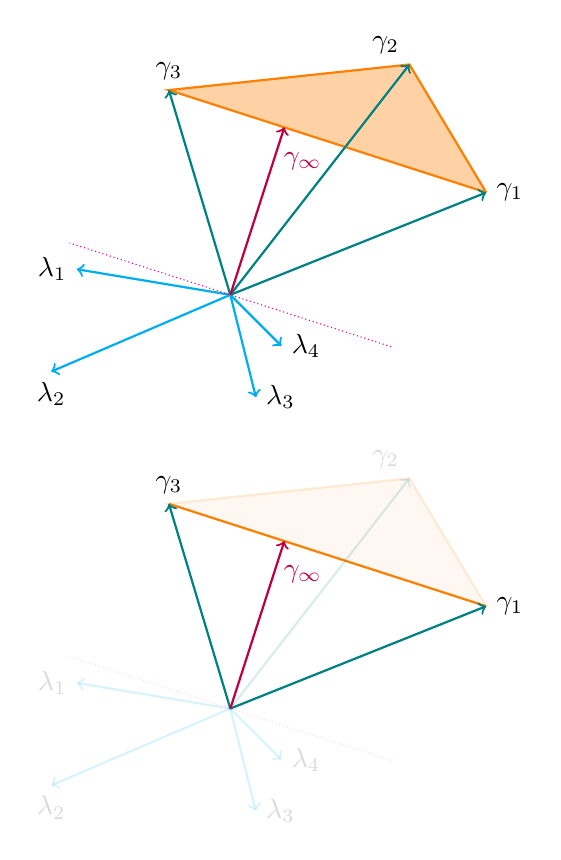
\begin{tikzpicture}[xscale=0.65,yscale=0.65,every node/.style={font=\normalsize}]

\begin{scope}
    \draw[orange, thick, fill=orange!35!white] (5,2) -- (3.5,4.5) -- (-1.2,4) -- (5,2);

    \draw[->, thick, teal] (0,0) -- (5,2) node[right,black]{$\gamma_1$};
    \draw[->, thick, teal] (0,0) -- (3.5,4.5) node[above left,black]{$\gamma_2$};
    \draw[->, thick, teal] (0,0) -- (-1.2,4) node[above,black]{$\gamma_3$};

    \draw[->, thick, cyan] (0,0) -- (-3,0.5) node[left,black]{$\lambda_1$};
    \draw[->, thick, cyan] (0,0) -- (-3.5,-1.5) node[below,black]{$\lambda_2$};
    \draw[->, thick, cyan] (0,0) -- (0.5,-2) node[right,black]{$\lambda_3$};
    \draw[->, thick, cyan] (0,0) -- (1,-1) node[right,black]{$\lambda_4$};

    \draw[rotate=atan(31/10), densely dotted, magenta] (0,-3.3) -- (0,3.3) node[above right]{};

    \draw[->, thick, purple] (0,0) -- (1120/1061,3472/1061) node[right,pos=0.8]{$\gamma_\infty$};
\end{scope}

\begin{scope}[yshift=-230pt]
    \draw[orange, thick, fill=orange!35!white, opacity=0.15] (5,2) -- (3.5,4.5) -- (-1.2,4) -- (5,2);
    \draw[orange, thick] (5,2) -- (-1.2,4);

    \draw[->, thick, teal] (0,0) -- (5,2) node[right,black]{$\gamma_1$};
    \draw[->, thick, teal, opacity=0.15] (0,0) -- (3.5,4.5) node[above left,black]{$\gamma_2$};
    \draw[->, thick, teal] (0,0) -- (-1.2,4) node[above,black]{$\gamma_3$};

    \draw[->, thick, cyan, opacity=0.15] (0,0) -- (-3,0.5) node[left,black]{$\lambda_1$};
    \draw[->, thick, cyan, opacity=0.15] (0,0) -- (-3.5,-1.5) node[below,black]{$\lambda_2$};
    \draw[->, thick, cyan, opacity=0.15] (0,0) -- (0.5,-2) node[right,black]{$\lambda_3$};
    \draw[->, thick, cyan, opacity=0.15] (0,0) -- (1,-1) node[right,black]{$\lambda_4$};

    \draw[rotate=atan(31/10), densely dotted, magenta, opacity=0.15] (0,-3.3) -- (0,3.3) node[above right]{};

    \draw[->, thick, purple] (0,0) -- (1120/1061,3472/1061) node[right,pos=0.8]{$\gamma_\infty$};
\end{scope}


\end{tikzpicture}

\end{document}